% network.tex
%

%begin{latexonly}
  \newcommand{\modgraphic}%
  {\centerline{\epsfig{file=figures/modgraphic.eps,width=2in}}}
%end{latexonly}
\begin{htmlonly}
  \newcommand{\srwindow}{%
  \htmladdimg[align=top,width="90%",alt="SCIRun Module Graphic"]
  {../figures/modgraphic.gif}}
\end{htmlonly}

%begin{latexonly}
  \newcommand{\moddialog}%
  {\centerline{\epsfig{file=figures/moddialog.eps,width=3in}}}
%end{latexonly}
\begin{htmlonly}
  \newcommand{\srwindow}{%
  \htmladdimg[align=top,width="90%",alt="SCIRun Module Dialog"]
  {../figures/moddialog.gif}}
\end{htmlonly}

\section{Working with Networks}
\label{sec:workwithnets}

This section describes how to create, save, open, execute, and edit
networks.

When started with no arguments the \command{scirun} command will create a
main window with a blank network pane.  The goal then is to create and
connect modules to form a network.


\subsection{Creating a Module}
\label{sec:creatingmodules}

To create a module select its name from one of the package (\eg \sr)
menus' category submenus.  The package menus may be accessed from the main
window's menu bar and from the network pane's popup menu.

You may activate the network pane's popup menu by clicking mouse button 3
while the mouse pointer is in the network pane (but not over a module or
connection).  

The popup menu contains a list of category submenus from the \sr\ package
and other installed packages.  And each category submenu provides
access to the modules within the category.

After creating a module its graphic ``front end'' will be created and
placed in the network pane.

\subsubsection{Anatomy of a Module}
\label{sec:modanatomy}

All modules are represented similarly by a graphic within the network pane.
See Figure~\ref{fig:modgraphic}. This graphical ``front end'' is the same
for all modules and consists of the following components:

\begin{description}
\item[Name] The module's name.
\item[Input ports] Zero or more input ports located on the top of the
  module.  Each port corresponds to a data type and each data type has a
  unique color.  Table~\ref{tab:portcolors} maps port colors to data types.
  Input ports connect to other modules' output ports.  Connections can only
  be made between ports of the same type.
\item[Output ports] Zero or more output ports located on the bottom of the
  module.  Output ports connect to other modules' input ports.  Every
  module has, of course, at least 1 input or 1 output port.
\item[UI button] Pressing the \button{UI} button displays the module's
  control dialog. Some modules have no such dialog. Some have very simple
  dialogs.  Some have very complex dialogs which allow elaborate control
  over the module.  Figure~\ref{fig:moddialog} shows the control dialog for
  \module{Show Fields} module.
\item[Progress bar] Shows the module's progress.
\item[Timer] Displays the amount of CPU time the module has consumed.
  Located to the left of the progress bar.
\item[Popup Menu] Pressing mouse button 3 while the mouse
  pointer is over a module gives access to the module's popup menu.  The
  popup menu gives access to the following items:
  \begin{description}
  \item[::Package\_Category\_Name\_Instance] This item is a label (not a
    selectable item).  It provides the module's name and the category and
    package to which to module belongs.  The Instance part is a unique
    number which distinguishes multiple instances of the same module.
  \item[\menuitem{Execute}] Executes the network.
  \item[\menuitem{Notes}] This item displays the module's note pad.  Use the note pad
    to document the purpose of the module in the current network.
  \item[\menuitem{Destroy}] Destroys the module.
  \item[\menuitem{Show Log}] Displays the module's message log.  Most modules will
    write messages to their log during the course of their execution.
  \item[\menuitem{Show Status}] This item is a toggle button which turns off/on the
    display of the progress indicator.  Turning off the progress indicator
    can help speed up the execution of complex networks.
  \end{description}
\end{description}

\begin{table}[htbp]
  \begin{center}
    \begin{tabular}{|l|l|}
      \hline
      \textbf{Data Type} & \textbf{Port Color} \\
      \hline
      Field & Yellow \\
      Field Set & Green \\
      Matricies & Blue \\
      Geometric Objects & Pink \\
      Color Maps & Purple \\
      Camera Path & Brown \\
      \hline
    \end{tabular}
    \caption{Data Types and their Port Colors}
    \label{tab:portcolors}
  \end{center}
\end{table}


\begin{figure}[htb]
  \begin{makeimage}
  \end{makeimage}
  \modgraphic
%  \centerline{\epsfig{file=figures/modgraphic.eps,width=6in}}
%    \framebox{\parbox[3in]{\columnwidth}{The\dotfill Figure\\
%    \vspace{2in}\\
%    With some \dotfill dummy text}}
  \caption{\label{fig:modgraphic} Module Graphic (\module{Show
      Fields} Module)}
\end{figure}

\begin{figure}[htb]
  \begin{makeimage}
  \end{makeimage}
  \moddialog
%  \centerline{\epsfig{file=figures/moddialog.eps,width=6in}}
%    \framebox{\parbox[3in]{\columnwidth}{The\dotfill Figure\\
%    \vspace{2in}\\
%    With some \dotfill dummy text}}
  \caption{\label{fig:moddialog} Module Control Dialog (\module{Show
      Fields} Module)}
\end{figure}

\subsection{Creating a Connection}
\label{sec:connectmods}

Mouse button 2 is used to connect the output (input) port of one module to the
input (output) port of another module.  

Position the mouse pointer over a module's input (output) port.  Then press
button 2 and drag the the mouse pointer towards another module's output (input)
port.   

When button 2 is first pressed the program shows all valid connections as
black lines.  It also draws one red colored connection which is the
connection that will be made if you stop the drag by releasing 
button 2.

Make the final connection by releasing button 2 when the pointer is over
the desired destination port or when the red colored connection is the
desired one.  The connection will be drawn using an appropriate data type
color.

You may connect a module's output port to the input ports of 1 or more
modules.

\subsection{Setting Module Properties}
\label{sec:setmodprops}

To change a module's properties click its \button{UI} button.  This will
display the module's control dialog.  Use this dialog to change the
module's properties.  Each module's reference documentation explains the
use of its control dialog.  Figure~\ref{fig:moddialog} shows the control
dialog for the ????? module.

\subsection{Executing a Network}
\label{sec:executenet}

``Network Execution'' means that 1 or more modules must be executed in a
coordinated fashion. The coordinated execution of modules is managed by
\sr{}'s \dfn{scheduler}.

\subsubsection{The Basics}

The scheduler is invoked when an event occurs that \dfn{triggers} a
module's execution.  The scheduler creates a list of all modules that must
executed in coordination with the triggered module. Modules
\dfn{upstream} (directly or indirectly) from the triggered module will be
put on the execution list if they have not previously executed.  And all
modules \dfn{downstream} from the triggered module will be put on the
list.  Once the scheduler determines which modules must be executed, it
executes them.

Network execution is mostly transparent.  That is, the events that trigger
module execution will usually be generated automatically while you work
(\eg by changing a module's property).  Sometimes though you must manually
generate a triggering event by choosing the \menuitem{Execute} item from a
module's popup menu.

\subsubsection{Details}

Each module executes in its own thread and blocks (waits) until its upstream
modules can supply it with data.  After a module completes its computation
it sends its results to its downstream modules.  This completes a module's
execution cycle.  Its next chance to recieve data from its input ports
and send data to its output ports won't arise until some event
causes it to be put on the scheduler's execution list again.  

This behavior prevents modules from computing in an iterative fashion,
sending intermediate results to their downstream modules.  This is because
downstream modules can't recieve these results until they are in their
execution cycle.  They would need to be executed each time the
upstream module posts an intermediate result.


\subsubsection{Intermediate Results}

Some modules are designed to be used in an interative fashion.  They send
data to their output ports in a special way.  They use a method called
\icode{send\_intermediate} to send the results of each iteration.  When
this method is used the scheduler (re)executes downstream modules each time
the upstream module posts its next result.  Downstream modules are
therefore able to receive the results of each iteration as soon as the
upstream module sends them.

Currently module \module{SolveMatrix} (from the \package(\sr) package and
\category{Math} category) is the only module that computes iteratively
using the \icode{send\_intermediate} method.

\subsubsection{Feedback Loops}

Some modules that are designed to be used in feedback loops (and if fact,
they can only be used this way).  Their output ports may be connected
directly or indirectly to their input ports.  These modules also use the
\icode{send\_intermediate} method.

The list of feedback modules is \module{DipoleSearch} and
\module{ConductivitySearch} from the \category{Inverse} category of the
\package{BioPSE} package and \module{BuildLeadField} from the
\category{LeadField} category of the \package{BioPSE} package.

\subsection{Deleting a Connection}
\label{sec:deleteconnections}

Delete a connection by pressing button 3 while the pointer is
over a connection.

\subsection{Selecting Modules}
\label{sec:selectmods}

A few operations (see \secref{Moving Module(s)}{sec:movemod} and
\secref{Destroying Module(s)}{sec:destroymod}) act on a group of
modules.  There are 2 ways to create a group of modules.

\begin{enumerate}
\item Press mouse button 2 while the pointer is in the network pane but not over
a module or a connection.  Then drag the mouse.  This will draw a box
outline.  Modules intersecting the box will be part of the group.  Release
button 2 to complete your selection.
\item Select the first module by clicking mouse button 2 while the pointer is
over a module.  Then add modules to the group by pressing (and holding
down) the \keyboard{control} key while you click on modules with button 2.
\end{enumerate}

Selected modules will be drawn in a slightly darker shade of grey.

You may mix selection methods -- you may always add modules the group by
pressing the control key while making selections using the above methods.
If you don't press the control key then the previous group will be
forgotton and a new one will be created.

\subsection{Moving Module(s)}
\label{sec:movemod}

Modules may be moved around in the network pane.  To move a module simply
press button 1 while the pointer is over a module and drag the module to
its new location.

Multiple modules may be moved at one time.  To do this first
\hyperref{select}{select (see Section~}{)}{sec:selectmods} 1 or more
modules. Then press button 1 while the pointer is over any one of the
modules in the selected group and then drag the modules to their new location.


\subsection{Destroying Module(s)}
\label{sec:destroymod}

Delete a module by selecting the \menuitem{Destroy} menu item from the
module's popup menu.

Multiple modules may be deleted at one time.  To do this first
\hyperref{select}{select (see Section~}{)}{sec:selectmods} 1 or more
modules. Then choose, from the popup menu of any one of the modules in the
selected group, the \menuitem{Destroy Selected} item.


\subsection{Documenting a Module}
\label{sec:docmodule}

It is often useful to document the purpose of a module within a network.
Each module maintains a note pad for this purpose.  You may edit the
module's note pad by selecting \menuitem{Notes} item from the module's
popup menu.  This will display the module's note pad editor.  This simple
editor allows you to write notes or otherwise document the use of the
module within the context of its network.

\subsection{Viewing a Module's Log}
\label{sec:viewmodslog}

Each module supports a message log.  The module may write error messages or
other types of messages to its log.  To view this log select the
\menuitem{Show Log} item from the module's popup menu.

\subsection{Documenting a Network}
\label{sec:docnetwork}

It is useful to document the purpose of a network.  You may use a network's
note pad for this purpose.  To edit the network's note pad select the
\menuitem{Add Info} item from the main window's \menu{File} menu.  This
will display the network's note pad editor.  This simple editor allows you
to write notes or otherwise document the purpose and use of the network.


\subsection{Saving a Network}
\label{sec:savenet}

\sr\ can save networks to files.  These network files have an extension of
\filename{.net} (although in the past they have also had .sr and .uin
extensions).  

To save a network select the \menuitem{Save} item from the main window's
\menu{File} menu.  A file browser dialog will prompt you for the
name (and location) of the network file.

Network files are actually \dfna{Tool Command Language}{TCL} scripts and
are editable.

\subsection{Opening a Network}
\label{sec:opennet}

To open a network file select the \menuitem{Open} item from the main
window's \menu{File} menu.   A file browser dialog will prompt you for the
name (and location) of the network file.

Note that opening a network file merges the network in the file with the
network in the network pane.  There is currently no way to ``close'' a
network and then open a new one -- you must quit and restart \sr\ to do
this.

\subsection{Navigating a Network}
\label{sec:navnetwork}

A complex network may not be entirely visible in the network pane.  You may
use the network pane's scroll bars to bring other parts of a network into
view.  Or you may use the navigation tool to view complex networks.

The navigation pane shows the entire ``network world.''  The small
rectangular region (outlined in black) within the navigation pane is the
network navigation tool and it is a window on the network world.  The
position of the navigation tool determines the part of the network that is
visible in the network pane.  To view other parts of the network, press
button 1 while the pointer is anywhere in the navigation pane -- this will
move the tool to the location of the pointer --  then drag the tool to the
new location.



%%% Local Variables: 
%%% mode: latex
%%% TeX-master: "usersguide"
%%% End: 
